\documentclass[14pt]{extarticle}
\usepackage{amsmath}
\usepackage{amssymb}
\usepackage{graphicx}
\graphicspath{ {../chap09/} }
\usepackage[top=1in, bottom=0.75in, left=0.75in, right=0.75in]{geometry}
\newcommand*{\Scale}[2][4]{\scalebox{#1}{\ensuremath{#2}}}%
% \usepackage{showframe}


\begin{document}

\section*{Math208 Discussion Outline for 10/29/2020}

\subsection{Homework and other due dates}
\begin{itemize}
\item Section 9.1 due 10/30
\item Section 9.2 due 11/3
\item Complete the Instruction Survey
\end{itemize}

\subsection{Questions}
\begin{itemize}
	\item Have you seen limits or derivatives before?
	\item Ask Questions
\end{itemize}

\subsection{Goals}
\subsubsection*{Section 9.1: Limits}
\begin{itemize}
	\item What is a limit?
	\item Describe polynomial and rational functions
	\item Analyzing limits
	\item Evaluating limits
	\item Identify indeterminate form limits
\end{itemize}

\subsubsection*{Section 9.2: Infinite Limits}
\begin{itemize}
	\item Identify and find infinite limits and vertical asymptotes
	\item Determine limits at infinity and horizontal asymptotes
\end{itemize}


\subsection{In class assignment}

\resizebox{15cm}{!}{
{Complete the Instruction Survey}
}


\cleardoublepage
\subsection*{Section 9.1: Limits}

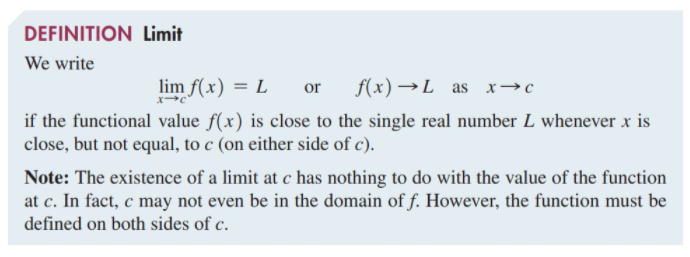
\includegraphics{9-1-1} \\
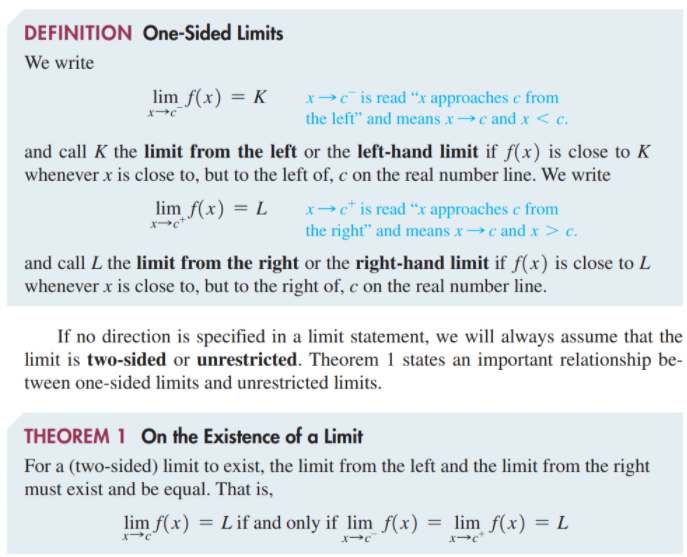
\includegraphics{9-1-2} \\
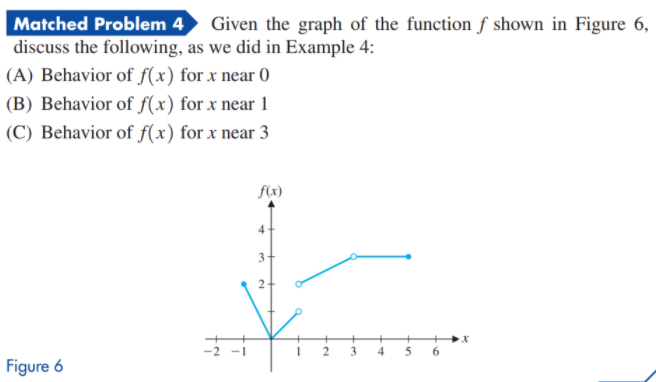
\includegraphics{9-1-3} \\
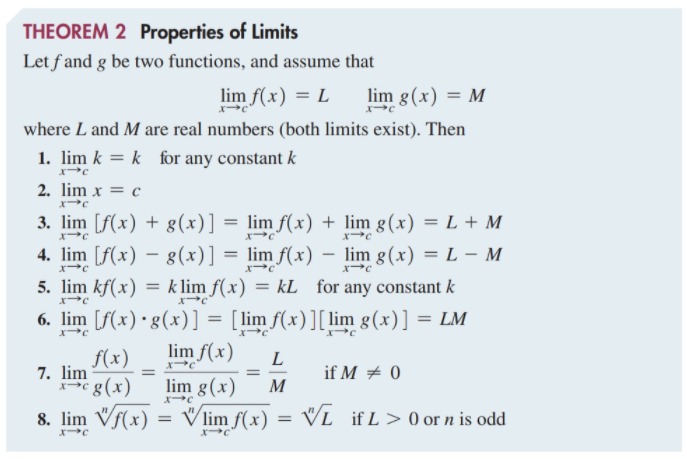
\includegraphics{9-1-4} \\
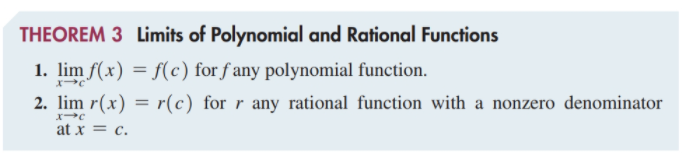
\includegraphics{9-1-5} \\
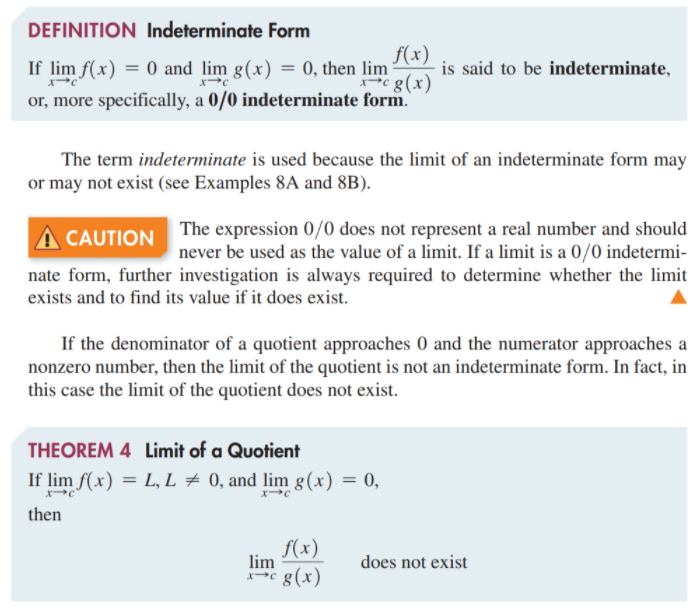
\includegraphics{9-1-6} \\
\begin{center}
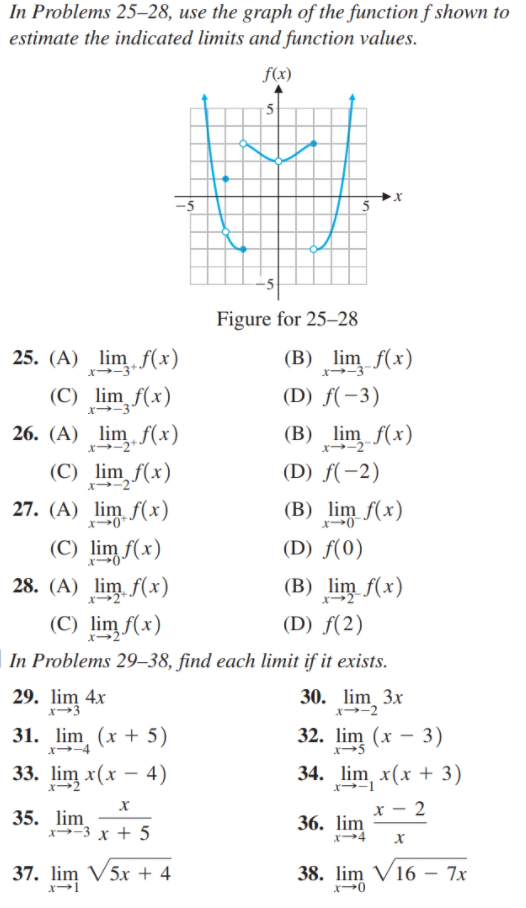
\includegraphics[width=0.7\linewidth]{9-1-7} \\
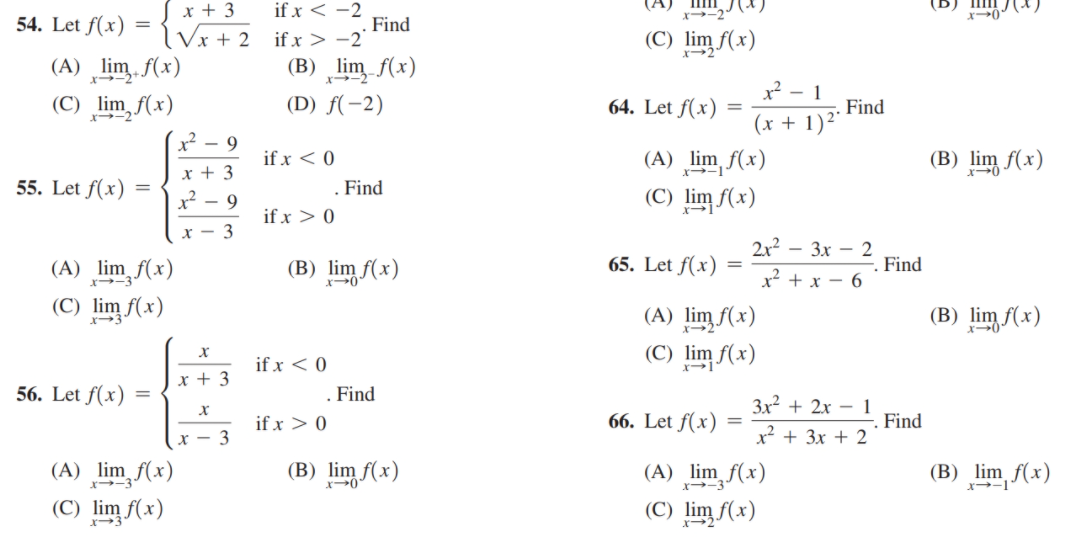
\includegraphics[width=1.1\linewidth]{9-1-8} \\
\end{center}

\cleardoublepage
\subsection*{Section 9.2: Infinite Limits}
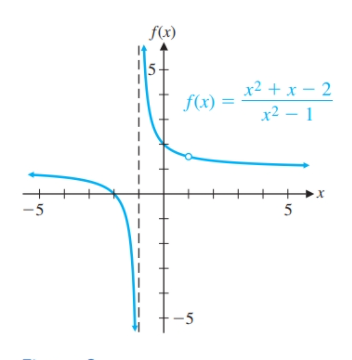
\includegraphics[width=0.4\linewidth]{9-2-1}
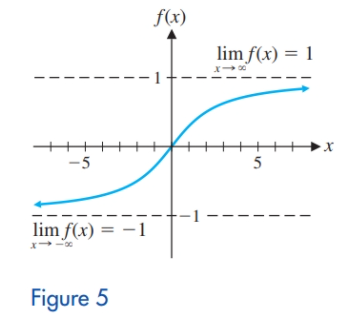
\includegraphics[width=0.4\linewidth]{9-2-4} 
\begin{center}
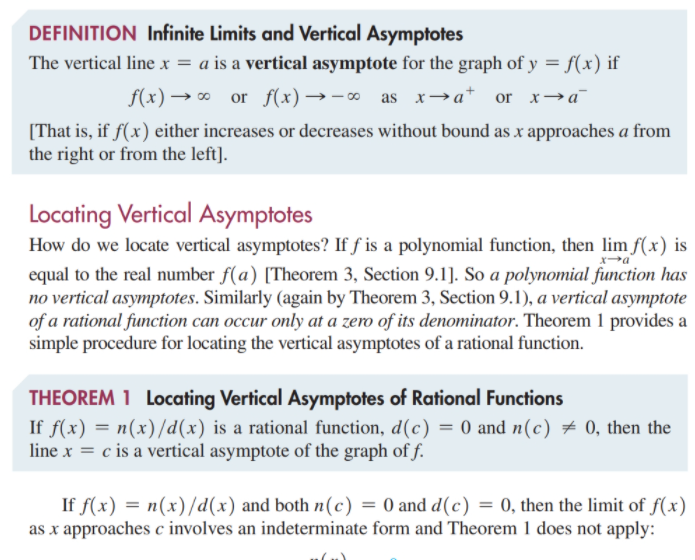
\includegraphics[width=1.0\linewidth]{9-2-2} \\
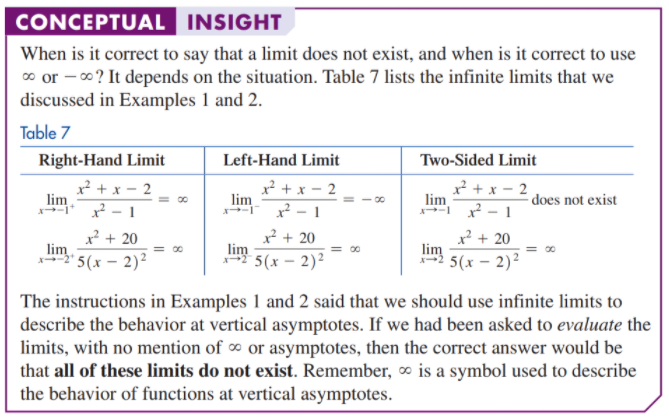
\includegraphics[width=0.9\linewidth]{9-2-3} \\
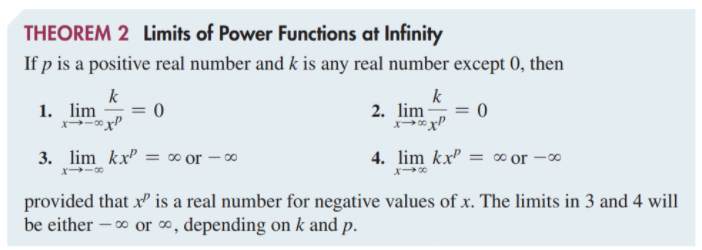
\includegraphics[width=0.9\linewidth]{9-2-5} \\
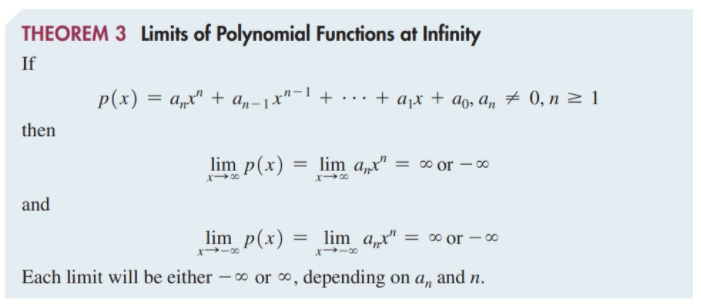
\includegraphics[width=0.9\linewidth]{9-2-6} \\
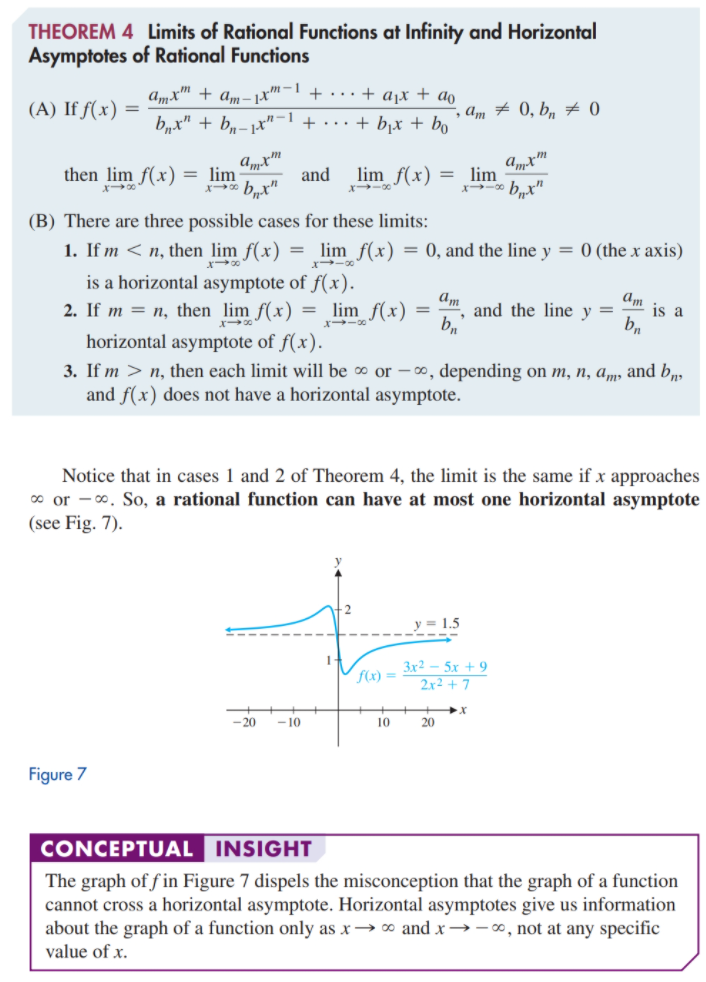
\includegraphics[width=0.9\linewidth]{9-2-7} \\

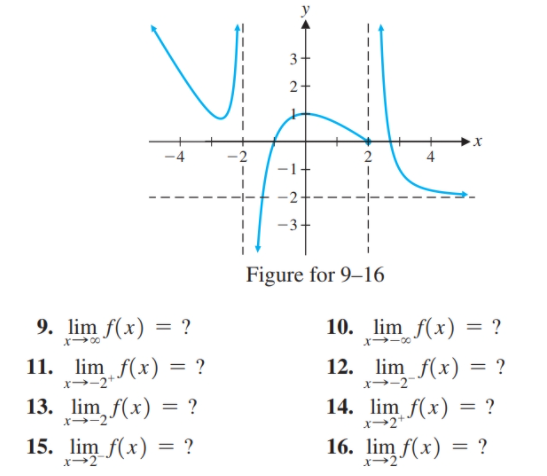
\includegraphics[width=0.8\linewidth]{9-2-8} \\
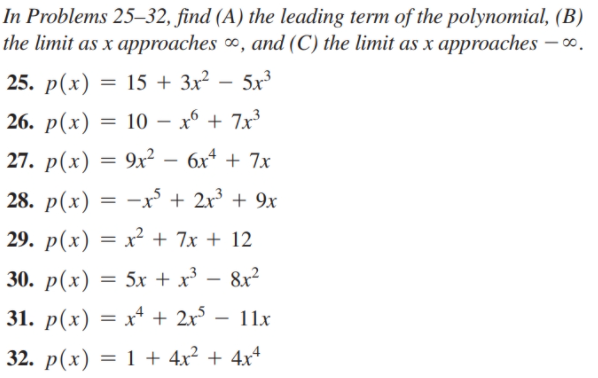
\includegraphics[width=0.8\linewidth]{9-2-9} \\
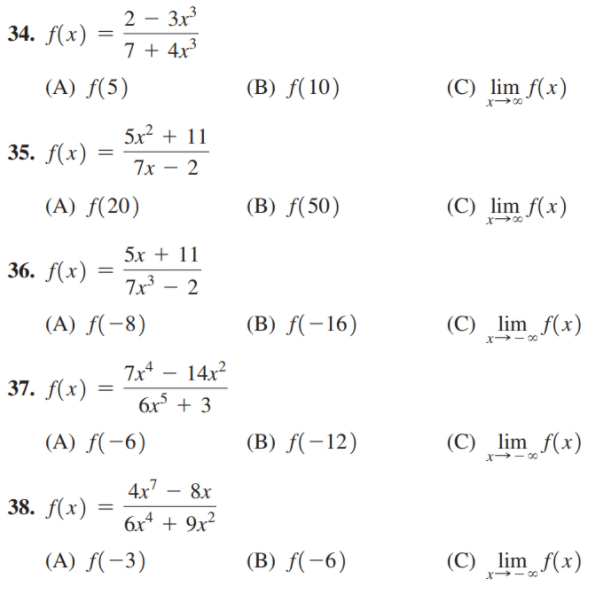
\includegraphics[width=0.9\linewidth]{9-2-10} \\
\end{center}




\end{document}
